\documentclass[11pt,a4paper]{ctexart}
\usepackage[a4paper,margin=1.78cm,headheight=15pt]{geometry}
\usepackage{amsmath,amssymb,mathtools,bm}
\usepackage{booktabs,longtable,tabularx,array}
\usepackage{enumitem}
\usepackage[most]{tcolorbox}
\usepackage{tikz}
\usetikzlibrary{arrows.meta,positioning,fit,calc}
\usepackage{pgfplots}
\pgfplotsset{compat=1.18}
\usepackage{xcolor}
\usepackage{fancyhdr}
\usepackage{hyperref}
\usepackage{microtype}

\newcolumntype{Y}{>{\raggedright\arraybackslash}X}
\newcolumntype{L}[1]{>{\raggedright\arraybackslash}p{#1}}
\setlength{\parindent}{2em}
\setlength{\parskip}{0.34em}
\setlength{\emergencystretch}{3em}
\renewcommand{\arraystretch}{1.22}
\setlength{\tabcolsep}{3pt}
\setlist[itemize]{itemsep=0.18em,topsep=0.35em,leftmargin=2em}
\setlist[enumerate]{itemsep=0.18em,topsep=0.35em,leftmargin=2em}

\definecolor{deep}{RGB}{42,58,73}
\definecolor{soft}{RGB}{245,247,249}
\definecolor{accent}{RGB}{104,76,55}
\definecolor{greenish}{RGB}{57,92,76}
\definecolor{warn}{RGB}{136,68,63}
\definecolor{purple}{RGB}{87,72,116}
\hypersetup{colorlinks=true,linkcolor=deep,urlcolor=accent,pdftitle={函数对象、表示与结构}}
\pagestyle{fancy}
\fancyhf{}
\lhead{\small\color{deep}\textbf{数学一 · 高等数学 Topic 01}}
\rhead{\small\color{deep}函数对象 · 表示 · 结构}
\cfoot{\small\thepage}
\renewcommand{\headrulewidth}{0.4pt}
\newtcolorbox{corebox}[1]{breakable,colback=soft,colframe=deep,title=\textbf{#1},boxrule=0.8pt,arc=2mm}
\newtcolorbox{methodbox}[1]{breakable,colback=white,colframe=greenish,title=\textbf{#1},boxrule=0.7pt,arc=1.5mm}
\newtcolorbox{warnbox}[1]{breakable,colback=white,colframe=warn,title=\textbf{#1},boxrule=0.7pt,arc=1.5mm}
\newtcolorbox{examplebox}[1]{breakable,colback=white,colframe=purple,title=\textbf{#1},boxrule=0.7pt,arc=1.5mm}
\newcommand{\kw}[1]{\textbf{\color{deep}#1}}
\providecommand{\tightlist}{}
\newcounter{none}

\begin{document}
\begin{center}
{\LARGE\textbf{函数对象、表示与结构}}\\[0.4em]
{\large 从“看见公式”到“确认对象与输入关系”}
\end{center}
\vspace{0.5em}

\begin{quote}
本册先解决一个比``怎么算''更早的问题：\textbf{当前到底是哪一个函数对象？它现在用什么方式表示？定义域、值域、单射/反函数，以及奇偶、周期、单调等性质，分别对应四问中的哪一种数学约束？}
\end{quote}

\begin{center}\rule{0.5\linewidth}{0.5pt}\end{center}

\setcounter{section}{-1}
\section{本册定位}\label{ux672cux518cux5b9aux4f4d}

本册是高等数学学科总图下的专题 01，是后续极限、微分、积分与函数展开共同依赖的函数对象入口。

\subsection{本册负责}\label{own}

本册独立负责：

\begin{itemize}
\tightlist
\item
  函数对象由哪些数据确定：定义域、对应规律，以及在需要时区分陪域与实际值域；表达式本身不能唯一确定函数对象；
\item
  显式、分段、隐式、参数式、图像等表示方式及其信息边界；
\item
  复合函数与反函数作为函数对象之间的基本操作，包括复合接口、单射/双射条件、单射限制的选择、主值分支为什么必要以及反函数的结构迁移；具体反解题型、主值代表的分段公式与局部技巧由同目录训练 Markdown 承接；
\item
  奇偶性、一般轴对称、一般中心对称，以及固定平移下的函数值关系；其中周期由 $f(x+T)=f(x)$ 定义，平移翻转关系 $f(x+L)=2b-f(x)$ 可进一步推出周期，纵向漂移关系则单独处理；
\item
  单调性、有界性、单射性等基础结构的语义与边界；
\item
  坐标平移/伸缩以后，函数自身结构的位置怎样改变；
\item
  两个反射结构为什么能够生成平移与周期；
\item
  任意函数的奇偶分解。
\end{itemize}

\subsection{调用与接口}\label{use-bridge}

本册\textbf{不拥有}以下传播规律：

\begin{itemize}
\tightlist
\item
  对称/周期结构怎样约束极限与连续；
\item
  求导以后奇偶、对称、周期怎样变化；
\item
  积分、变上限积分以后结构怎样变化；
\item
  泰勒 / 傅里叶展开怎样读取函数结构。
\end{itemize}

这些跨专题的传播规律统一由
\href{../50_桥梁专题/H-B01_函数结构在运算中的传播/README.md}{H-B01｜函数结构在运算中的传播}
承担；极限、微分、积分、展开本身仍由对应专题拥有。

本册也不拥有``用导数判单调/极值/凹凸''的机制，该部分属于
\href{../04_局部到整体_中值定理与函数形状/README.md}{专题04｜局部到整体：中值定理与函数形状}。

\begin{center}\rule{0.5\linewidth}{0.5pt}\end{center}

\section{根本问题：为什么不能把函数当成一个公式？}\label{ux6839ux672cux95eeux9898ux4e3aux4ec0ux4e48ux4e0dux80fdux628aux51fdux6570ux5f53ux6210ux4e00ux4e2aux516cux5f0f}

数学一里最常见的函数写法是

\[
y=f(x).
\]

这很容易形成一个危险的直觉：

\begin{quote}
``看见一个解析式，就已经知道函数是什么。''
\end{quote}

但一个函数首先是\textbf{允许哪些输入，以及每个允许输入对应哪个输出}。

例如

\[
f(x)=\frac{x^2-1}{x-1},\qquad x\ne1
\]

与

\[
g(x)=x+1,\qquad x\in\mathbb R
\]

虽然在 \(x\ne1\)
时函数值完全相同，却不是同一个函数对象，因为它们的定义域不同。

如果把前式直接约成 \(x+1\) 而忘记
\(x\ne1\)，代数式变简单了，但对象已经被偷偷改变。

因此，本册的母问题不是``函数有哪些性质''，而是：

\begin{quote}
\textbf{怎样确定当前函数对象；怎样在保持定义域与对应关系不变的前提下切换表示；又怎样由输入之间的关系推出相应的函数值关系？}
\end{quote}

\begin{center}\rule{0.5\linewidth}{0.5pt}\end{center}

\section{分析协议：对象 → 表示 → 输入关系 → 输出关系}\label{ux6bcdux6a21ux578bux5bf9ux8c61-ux8868ux793a-ux8f93ux5165ux5173ux7cfb-ux8f93ux51faux5173ux7cfb}

四问是本册的总坐标系；下面这条链只用于展开一个具体问题时组织分析顺序，不是另一套并列母模型：

\[
\boxed{
\text{确认函数对象}
\to
\text{选择或切换表示}
\to
\text{建立合法的输入关系}
\to
\text{比较对应输出}
\to
\text{读取结构}
}
\]

这里的箭头表示\textbf{分析顺序}，不是数学对象之间的因果生成关系。

它的自然语言版本是：

\begin{enumerate}
\def\labelenumi{\arabic{enumi}.}
\tightlist
\item
  \textbf{对象}：哪些 \(x\) 允许进入？每个 \(x\) 对应什么值？
\item
  \textbf{表示}：当前写法是否最适合暴露结构？换写法会不会丢分支、增解或改变定义域？
\item
  \textbf{输入关系}：现在比较的是 \(x\) 与 \(-x\)、\(x\) 与
  \(2a-x\)、\(x\) 与 \(x+T\)，还是两个满足 \(x_1<x_2\) 的输入？
\item
  \textbf{输出关系}：对应函数值相等、反号、和为常数、保持顺序，还是被限制在某个范围？
\item
  \textbf{结构}：由此再命名为轴对称、中心对称、奇偶、周期、单调等由输入关系刻画的结构。单射与有界性分别由第三问的原像唯一性和第二问的像集范围处理。
\end{enumerate}

一句话压缩：

\[
\boxed{
\text{对称、周期、单调等关系型结构，可以由输入关系与对应函数值关系统一描述。}
}
\]

这比直接背``奇函数公式、偶函数公式、周期函数公式''更有生成力。

\subsection{总坐标系：四个问题统一函数的基础性质}

把函数画成最朴素的一条箭头：

\[
x\in D\xrightarrow{\ f\ }y.
\]

第一章真正需要反复检查的，可以压缩为四个数学问题：

\begin{enumerate}
\tightlist
\item
  \textbf{输入合法性（定义域）}：哪些 \(x\) 属于定义域 \(D\)？
\item
  \textbf{输出可达性（值域）}：哪些 \(y\) 属于像集 \(f(D)\)？
\item
  \textbf{原像唯一性（单射性）}：对给定 \(y\)，原像集 \(f^{-1}(\{y\})\) 中有多少个元素？当陪域取实际值域 \(f(D)\) 时，这一问也决定逆映射是否存在。
\item
  \textbf{输入关系在映射下的保持与变换}：已知两个合法输入 \(x_1,x_2\) 满足某种关系时，\(f(x_1),f(x_2)\) 满足什么关系？奇偶、一般对称、周期与单调都属于这一问题。
\end{enumerate}

第四问可以统一写成

\[
\boxed{
x_1\mathrel{R_D}x_2
\quad\Longrightarrow\quad
f(x_1)\mathrel{R_B}f(x_2),
}
\]

其中 \(R_D\) 表示输入之间的关系，\(R_B\) 表示对应输出之间的关系。例如：

\begin{itemize}
\tightlist
\item
  轴对称：\(x_1+x_2=2a\Rightarrow f(x_1)=f(x_2)\)；
\item
  中心对称：\(x_1+x_2=2a\Rightarrow f(x_1)+f(x_2)=2b\)；
\item
  周期：\(x_2-x_1=T\Rightarrow f(x_2)=f(x_1)\)；
\item
  单调递增：\(x_1<x_2\Rightarrow f(x_1)\le f(x_2)\)，严格递增时右侧改为严格不等式。
\end{itemize}

这样第四问不是一个含糊的概括词，而是在研究\textbf{输入关系经过映射以后，对应的输出关系是什么}。

对一个固定输出 \(y\)，定义它在 \(f\) 下的\textbf{原像集}

\[
P_y=f^{-1}(\{y\})=\{x\in D:f(x)=y\}.
\]

这里的 \(f^{-1}(\{y\})\) 表示集合的原像，不要求反函数已经存在。它就是方程 \(f(x)=y\) 在定义域 \(D\) 中的全部解。于是值域、单射和双射都可以用原像集的元素个数统一表述：

\[
\boxed{
y\in f(D)
\Longleftrightarrow
P_y\ne\varnothing
}
\]

说明\textbf{值域问的是``至少有没有一个原输入''}；

\[
\boxed{
f:D\to B\text{ 单射}
\Longleftrightarrow
\forall y\in B,\ \lvert P_y\rvert\le1
}
\]

说明\textbf{单射要求每个输出至多有一个原像}；若把陪域记为 \(B\)，则

\[
\boxed{
f:D\to B\text{ 为双射}
\Longleftrightarrow
\forall y\in B,\ \lvert P_y\rvert=1.
}
\]

因此，当 $f:D\to B$ 为双射时，可以把每个 $y\in B$ 唯一对应的原像定义为 $f^{-1}(y)$，从而得到逆映射。

几何上也因此得到两个完全不同的检查：

\begin{itemize}
\tightlist
\item
  \textbf{竖线检查}：同一个 \(x\) 是否只对应一个 \(y\)？它检查当前关系是不是函数；
\item
  \textbf{横线检查}：同一个 \(y\) 是否至多对应一个 \(x\)？它检查函数是否单射；若把目标集合取为实际值域 \(f(D)\)，单射就保证逆映射存在。
\end{itemize}

这套``输入合法性—输出可达性—原像唯一性—输入关系的映射规律''是本册的总坐标系。后面的定义域、值域、单射与反函数、对称、周期和单调，都可以定位到其中一问；复合与表示变换则属于操作层，会调用其中一问或多问。

\begin{examplebox}{最小母例：只用四问重新读懂 \(f(x)=x^2\)}
先不背“偶函数”“无反函数”这些标签，只沿四问走一遍。

\textbf{第一问：输入是否合法？} 若函数对象是
\[
f:\mathbb R\to\mathbb R,\qquad f(x)=x^2,
\]
则所有实数都允许输入，所以定义域是 \(\mathbb R\)。

\textbf{第二问：哪些输出可达？} 因为 \(x^2\ge0\)，而每个 \(y\ge0\) 都可由 \(x=\sqrt y\) 取得，所以实际值域是
\[
R_f=[0,+\infty).
\]

\textbf{第三问：给定输出的原像是否唯一？} 对 \(y>0\)，方程
\[
x^2=y
\]
在原定义域中有两个解 \(x=\pm\sqrt y\)，即 \(\lvert P_y\rvert=2\)。因此全实轴上的 \(f\) 不是单射，没有全局反函数。若把定义域限制为 \([0,+\infty)\)，则对每个 \(y\ge0\) 都有唯一原像，才得到反函数 \(f^{-1}(y)=\sqrt y\)。

\textbf{第四问：输入关系经过映射后变成什么输出关系？} 对互为相反数的两个输入 \(x,-x\)，
\[
f(-x)=(-x)^2=x^2=f(x),
\]
所以输出不变，这才正式命名为偶函数结构。

因此定义域、值域、单射/反函数、偶性不是四条互不相干的知识，而是同一个函数对象在四个问题下的四个回答。
\end{examplebox}

\begin{center}\rule{0.5\linewidth}{0.5pt}\end{center}

\section{函数对象：先确定什么不能被变形偷偷改掉}\label{ux51fdux6570ux5bf9ux8c61ux5148ux786eux5b9aux4ec0ux4e48ux4e0dux80fdux88abux53d8ux5f62ux5077ux5077ux6539ux6389}

\subsection{工作对象}\label{ux5de5ux4f5cux5bf9ux8c61}

在数学一的一元实函数语境中，更完整地可以把函数写成

\[
f:D\to B,\qquad B\subseteq\mathbb R,
\]

其中：

\begin{itemize}
\tightlist
\item
  \(D\) 是\textbf{定义域}：允许进入函数的输入集合；
\item
  \(B\) 是\textbf{陪域}：事先声明允许输出落入的目标集合；
\item
  \(f\) 给出\textbf{对应规律}：每个 \(x\in D\) 对应唯一函数值 \(f(x)\)；
\item
  \textbf{值域}是实际被取得的输出集合 \[
  R_f=f(D)=\{f(x):x\in D\}\subseteq B.
  \]
\end{itemize}

必须把\textbf{陪域}与\textbf{值域}分开：前者是声明的目标集合，后者是实际到达的集合。满射问的是
\(R_f=B\)，而求通常意义下的反函数时，反函数真正允许输入的集合是原函数实际值域
\(R_f\)。

在本课程通常的``实函数''工作语境中，判断两个函数对象是否相同，最常用的检查是：

\[
\boxed{\text{定义域相同}+\text{定义域内逐点函数值相同}.}
\]

若题目把函数明确写成映射 \(f:D\to B\) 并讨论满射、双射等性质，则陪域 \(B\) 也属于当前映射对象的数据，不能再省略。只看最终解析式始终不够。

\subsection{保持同一函数对象时必须保持什么}\label{ux5bf9ux8c61ux8eabux4efdux7684ux4e0dux53d8ux91cf}

当我们说``只是换一种表示，没有改变函数对象''时，至少要保护：

\begin{enumerate}
\def\labelenumi{\arabic{enumi}.}
\tightlist
\item
  原来的允许输入没有被无意扩大或缩小；
\item
  每个保留下来的输入对应同一个输出；
\item
  若表示引入参数或分支，覆盖范围没有丢失；
\item
  若后续推理依赖方向、分支或一一对应性，这些信息没有被消掉。
\end{enumerate}

这就是专题01最基础的合法性要求。

\subsection{定义域不是附属条件：它是所有定义条件的交集}

定义域题最稳的做法不是``凭经验看哪里不能取''，而是逐层写出每个运算有定义所要求的条件。若一个表达式同时要求若干条件
\(C_1,C_2,\ldots,C_m\)，则

\[
\boxed{
D_f=C_1\cap C_2\cap\cdots\cap C_m.
}
\]

常见定义条件包括：

\begin{itemize}
\tightlist
\item
  分母：\(q(x)\ne0\)；
\item
  偶次根式：被开方量 \(r(x)\ge0\)；
\item
  对数：真数 \(u(x)>0\)；
\item
  \(\arcsin,\arccos\)：内层值必须落在 \([-1,1]\)；
\item
  \(\tan u\)：要求 \(\cos u\ne0\)；\(\cot u\)：要求 \(\sin u\ne0\)；
\item
  复合 \(f(g(x))\)：既要 \(x\in D_g\)，又要 \(g(x)\in D_f\)。
\end{itemize}

真正容易出错的不是列条件，而是\textbf{不同条件之间可能存在蕴含、交叠或矛盾}。例如

\[
h(x)=\arcsin\bigl(\ln(x-1)\bigr).
\]

不能只写 \(x>1\)。外层 \(\arcsin\) 继续要求

\[
-1\le\ln(x-1)\le1,
\]

于是

\[
e^{-1}\le x-1\le e,
\]

最终

\[
\boxed{D_h=[1+e^{-1},\,1+e].}
\]

这里外层给出的定义条件已经自动保证了对数真数为正。这个例子体现了复合函数定义域最稳定的执行顺序：

\[
\boxed{
\text{从内到外列定义条件}
\to
\text{全部拉回到原变量}
\to
\text{最后取交集并化简}.
}
\]

\begin{warnbox}{定义域边界：化简成功不等于原定义条件消失}
若原对象已经要求``分母不为零''、``真数为正''或某个分支条件，即使后续代数变形把相应因子约掉、平方掉或消元掉，这些原始定义条件仍要保留，除非已经证明新条件与原条件完全等价。
\end{warnbox}

\begin{center}\rule{0.5\linewidth}{0.5pt}\end{center}

\section{表示不是对象：换写法之前先问``信息有没有丢''}\label{ux8868ux793aux4e0dux662fux5bf9ux8c61ux6362ux5199ux6cd5ux4e4bux524dux5148ux95eeux4fe1ux606fux6709ux6ca1ux6709ux4e22}

同一个数学对象可以有不同表示；反过来，一个看起来像``方程''的东西也不一定已经定义了一个全局函数。

\subsection{显式表示}\label{ux663eux5f0fux8868ux793a}

\[
y=f(x).
\]

优点是输入、输出关系直接；缺点是有些几何对象无法在整个区域内写成单值
\(y=f(x)\)。

\subsection{分段表示}\label{ux5206ux6bb5ux8868ux793a}

\[
f(x)=
\begin{cases}
f_1(x),&x\in D_1,\\
f_2(x),&x\in D_2.
\end{cases}
\]

分段函数首先是\textbf{一个函数对象}，不是几段互不相干的公式。研究连续、奇偶、单调或值域时，都必须把分界点与各段定义域一起维护。

\subsection{隐式关系}\label{ux9690ux5f0fux5173ux7cfb}

\[
F(x,y)=0
\]

首先描述的是 \(x,y\) 之间的\textbf{关系}，不自动等于一个全局函数
\(y=f(x)\)。

例如

\[
x^2+y^2=1
\]

对同一个 \(x\in(-1,1)\) 通常有两个 \(y\)，所以整圆不能直接当成单值函数
\(y=f(x)\)。只有选定上半圆或下半圆等分支以后，才得到相应函数。

因此：

\[
\boxed{\text{隐式方程}\neq\text{全局单值函数}.}
\]

\subsection{参数表示}\label{ux53c2ux6570ux8868ux793a}

\[
x=x(t),\qquad y=y(t).
\]

参数式直接表示的是一条由参数生成的轨迹。使用时必须检查：

\begin{itemize}
\tightlist
\item
  参数区间覆盖了多少对象；
\item
  是否重复经过同一点；
\item
  是否保留了走向；
\item
  能否在当前区间消去参数得到单值 \(y=f(x)\)。
\end{itemize}

``能够消元''不等于``消元后没有信息损失''。

\subsection{表示变换最常见的四类失真}\label{ux8868ux793aux53d8ux6362ux6700ux5e38ux89c1ux7684ux56dbux7c7bux5931ux771f}

\subsubsection{失真
A：约分扩大定义域}\label{ux5931ux771f-aux7ea6ux5206ux6269ux5927ux5b9aux4e49ux57df}

\[
\frac{x^2-1}{x-1}=x+1
\]

只在 \(x\ne1\) 的原定义域内成立。

\subsubsection{失真
B：平方引入额外分支}\label{ux5931ux771f-bux5e73ux65b9ux5f15ux5165ux989dux5916ux5206ux652f}

从

\[
\sqrt{x}=x-2
\]

两边平方得到的方程只是候选条件，必须回代原式与原定义域。

\subsubsection{失真
C：消元丢掉参数分支或方向}\label{ux5931ux771f-cux6d88ux5143ux4e22ux6389ux53c2ux6570ux5206ux652fux6216ux65b9ux5411}

参数式变成笛卡尔方程后，可能只保留轨迹集合，却丢掉覆盖次数和方向信息。

\subsubsection{失真
D：把局部分支误当全局对象}\label{ux5931ux771f-dux628aux5c40ux90e8ux5206ux652fux8befux5f53ux5168ux5c40ux5bf9ux8c61}

反三角函数、隐函数、反函数都常需要先限制区间，再获得单值分支。

所以表示变换的固定检查句是：

\begin{quote}
\textbf{新表示覆盖的还是原来的对象吗？有没有增加、遗漏或合并本来不同的分支？}
\end{quote}

\subsection{基本函数族不是图像表：把它们当成结构原型}

基本初等函数值得记，不是因为考试要求默写若干曲线，而是因为后面大量复杂函数都由这些原型经过\textbf{复合、平移、伸缩、限制分支和四则运算}生成。最有用的记忆单位应是

\[
\boxed{
\text{定义域}
+\text{实际值域}
+\text{最核心结构}
+\text{原像是否唯一}
}.
\]

\begin{center}
\begin{tabularx}{\linewidth}{L{2.7cm}L{3.2cm}L{3.7cm}Y}
\toprule
函数原型 & 定义域 / 值域 & 核心结构 & 单射性与反函数 \\
\midrule
\(x^{2m}\), \(m=1,2,\ldots\) & \(\mathbb R\to[0,+\infty)\) & 偶；\(f(x)=f(-x)\) & 在 \(\mathbb R\) 上非单射；限制到任一半轴后单射 \\
\(x^{2m+1}\), \(m=0,1,\ldots\) & \(\mathbb R\to\mathbb R\) & 奇；严格递增 & 在 \(\mathbb R\) 上双射，反函数为奇次根 \\
\(a^x\), \(a>0,a\ne1\) & \(\mathbb R\to(0,+\infty)\) & 始终为正；\(a>1\) 增，\(0<a<1\) 减 & 该映射为双射；反函数为 \(\log_a x\) \\
\(\log_a x\), \(a>0,a\ne1\) & \((0,+\infty)\to\mathbb R\) & 定义域要求 \(x>0\)；单调方向由 \(a\) 决定 & 该映射为双射；反函数为 \(a^x\) \\
\(\sin x,\cos x\) & \(\mathbb R\to[-1,1]\) & 有界、周期、重复取值 & 在 \(\mathbb R\) 上非单射；反三角函数来自限制后的主值分支 \\
\(\tan x\) & 去掉 \(\pi/2+k\pi\) 后取遍 \(\mathbb R\) & 每个连续分支严格递增，周期为 \(\pi\) & 每个连续分支到 \(\mathbb R\) 为双射；标准主支的反函数为 \(\arctan\) \\
\(\lvert x\rvert\) & \(\mathbb R\to[0,+\infty)\) & \(f(x)=f(-x)\)，在 \(\mathbb R\) 上非单射 & 限制到任一半轴后单射 \\
\bottomrule
\end{tabularx}
\end{center}

这里最值得形成的不是七条孤立曲线，而是三类原像结构：

\begin{itemize}
\tightlist
\item
  \textbf{单射型}：如奇次幂、指数、对数，对每个 \(y\in f(D)\)，原像集 \(f^{-1}(\{y\})\) 恰含一个元素；
\item
  \textbf{多原像型}：如偶次幂、绝对值，对某些输出存在两个不同原像，因此原函数在全定义域上非单射；
\item
  \textbf{周期重复型}：如非恒定三角函数，若 \(T\) 是周期，则 \(x\) 与 \(x+kT\) 取得同一函数值，从而在完整周期域上非单射。
\end{itemize}

反函数与分支选择因此可以统一到第三问“原像唯一性”；周期与对称则属于第四问“输入关系的映射规律”。它们之间可以发生联系，但不应混成同一个概念。

\begin{center}\rule{0.5\linewidth}{0.5pt}\end{center}

\section{复合与反函数：函数不是公式拼接，而是映射之间的连接}\label{ux590dux5408ux4e0eux53cdux51fdux6570ux51fdux6570ux4e0dux662fux516cux5f0fux62fcux63a5ux800cux662fux6620ux5c04ux4e4bux95f4ux7684ux8fdeux63a5}

\begin{corebox}{阅读层次：先抓“连接与信息”，再练反解技巧}
这一节内容较多，但第一次建立心智模型时不应平均用力。先只抓两件事：

\[
\boxed{
\text{复合}=\text{输出必须能合法交给下一层}
\qquad
\text{求逆}=\text{原函数必须在当前定义域上单射}
}
\]

掌握这两个对象级判据以后，再把后面的指数换元、共轭、平方筛支、反三角主值、分段反解等看成\textbf{“怎样把唯一原输入具体恢复出来”的表示技巧}。这样即使忘掉某个反函数公式，也不会把“不会反解”误判成“反函数不存在”。
\end{corebox}

\subsection{复合函数}\label{ux590dux5408ux51fdux6570}

若

\[
x\xrightarrow{g}u\xrightarrow{f}y,
\]

则

\[
(f\circ g)(x)=f(g(x)).
\]

真正关键的是接口是否合法：\(g(x)\) 必须落进 \(f\) 的定义域。

因此

\[
\boxed{
D_{f\circ g}=\{x\in D_g:g(x)\in D_f\}.
}
\]

这条定义域公式比``先算里面再算外面''更重要，因为它规定了两个函数什么时候真的能够连接。

复合后的奇偶、周期等结构不在这里重复展开；它们统一在后文“结构怎样在函数代数内部组合？”中处理。那里只保留一个问法：\textbf{目标输入变换先使内函数满足什么关系；把该关系代入外函数后，复合函数的函数值关系是什么？}

\subsection{反函数：核心不是换字母，而是恢复输入}\label{ux53cdux51fdux6570}

反函数解决的根本问题是：\textbf{只知道输出，能否唯一恢复原来的输入？}

若 \(f:D\to f(D)\) 在 \(D\) 上单射，则每个 \(y\in f(D)\) 都只来自一个
\(x\in D\)，于是可以定义

\[
f^{-1}:f(D)\to D,
\qquad
f^{-1}(y)=x\Longleftrightarrow f(x)=y.
\]

这里可以把截图里常见的“一个 \(x\) 对应一个 \(y\)，一个 \(y\) 对应一个 \(x\)”拆成两层责任：

\begin{itemize}
\tightlist
\item
  “每个允许的 \(x\) 对应唯一 \(y\)”只是\textbf{它是一个函数}；
\item
  “每个实际输出 \(y\) 至多有一个原像”才是\textbf{单射}。
\end{itemize}

如果把函数写成 \(f:D\to B\)，并要求反函数定义在整个给定陪域 \(B\) 上，那么还必须要求每个 \(y\in B\) 都被取到，即 \(f\) 对 \(B\) 满射；此时需要双射。若像本册一样把目标集合直接写成实际值域 \(f(D)\)，满射到 \(f(D)\) 自动成立，所以存在反函数的关键只剩单射。

\begin{corebox}{单射性是反函数存在的核心条件}
若存在
\[
x_1\ne x_2,
\qquad
f(x_1)=f(x_2),
\]
则同一个输出具有至少两个原像，原函数不是单射，因此不能在整个当前定义域上定义反函数。

所以限制定义域、选择严格单调分支、规定反三角函数的主值区间，数学上的共同目的都是：\textbf{把原函数限制为单射，使每个 \(y\in f(D)\) 具有唯一原像。}

直观地说，只有这样才能由输出唯一确定原输入；但正式判据始终是单射性。
\end{corebox}

因此

\[
\boxed{
D_{f^{-1}}=f(D),
\qquad
R_{f^{-1}}=D
}
\]

并且

\[
\boxed{
f^{-1}(f(x))=x,
\qquad
f(f^{-1}(y))=y.
}
\]

更不容易混淆定义域的写法是

\[
\boxed{
f^{-1}\circ f=I_D,
\qquad
f\circ f^{-1}=I_{f(D)},
}
\]

其中 \(I_A\) 表示集合 \(A\) 上的恒等映射。这样就不会被两边都写成字母 \(x\) 的记号迷惑：第一条恒等式从原定义域 \(D\) 出发，第二条从原值域 \(f(D)\) 出发。

这里第二个恒等式中的 \(y\) 必须属于 \(f(D)\)。反函数不是把符号
\(x,y\) 交换一下；交换字母只是最后的记号整理，真正的数学任务是从方程
\(y=f(x)\) 中\textbf{唯一解回原输入}。

所以第一问题永远是

\[
\boxed{\text{当前定义域上，}f\text{ 是否单射？}}
\]

在区间上，\textbf{严格单调}是保证单射、从而建立反函数的常用充分条件；但
若目标集合取实际值域 \(f(D)\)，则 \(f:D\to f(D)\) 存在逆映射当且仅当 \(f\) 在 \(D\) 上单射；若题目固定陪域 \(B\)，则必须进一步要求满射，即 \(f:D\to B\) 为双射。严格单调只是区间上保证单射的常用充分条件，不能与单射或双射的定义混同。尤其不要把“单调不减/单调不增”机械等同于反函数存在：常函数在区间上单调不减且单调不增，却不是单射。

\subsection{从存在性到具体反解：正文只保留接口}

反函数的知识层顺序只有三层：

\[
\boxed{
\text{原函数是否单射}
\to
\text{选定双射分支与值域}
\to
\text{在保持定义域、符号与分支条件的前提下恢复输入}
}.
\]

其中前两层决定\textbf{反函数是否作为映射存在}，第三层才是\textbf{如何写出它的表示}。指数换元、共轭、平方筛支、逐段反解等具体表示策略已经分流到本专题训练文档《反函数》，正文不再维护一份并行题型流程。

核心不变量仍是：

\[
\boxed{
\text{反解可以改变表示，但不能改变``每个输出对应哪个唯一原输入''。}
}
\]

\subsection{反解机制：表示可以换，但必须保持原定义域与分支条件}

具体反解会出现线性移项、分式收集、开方、取对数、指数换元、共轭、平方、反三角与逐段反解等不同外观。正文不再逐类维护题型解法，只保留统一机制：

\[
\boxed{
\text{把 }y=f(x)\text{ 改写成更容易恢复 }x\text{ 的表示}
\quad\text{同时持续保留定义域、符号与分支条件}
}
\]

任何在缺少附加条件时并非双向等价的代数操作，都只能生成\textbf{候选输入}；原定义域、符号与分支条件决定哪些候选仍满足原方程。最小母例 $x^2$ 已在前文跑通这一逻辑；线性、分式、指数、根式等完整反解谱系统一由训练文档《反函数》承接。

\subsubsection{存在性与表示能力必须分开}

例如 $f(x)=x+e^x$ 在 $\mathbb R$ 上严格递增，因此在 $\mathbb R$ 上单射，从而 $f:\mathbb R\to f(\mathbb R)$ 存在逆映射；即使当前课程工具不能把方程 $y=x+e^x$ 轻易改写成一个熟悉的初等闭式，也不影响逆映射存在。因此

\[
\boxed{\text{反函数存在}\neq\text{能够写成熟悉闭式公式}.}
\]

具体指数换元、共轭、根式平方与分段反解的完整母题已移入训练文档《反函数》；反三角主值分支与复合则由《反三角主值与复合》承接。

\subsection{主值分支：反三角函数不是把周期函数整体倒过来}

三角函数把反函数里最容易混淆的一层暴露得最彻底：\textbf{原来的周期函数并不全局单射，所以所谓反三角函数，实际上是某个指定单射分支的反函数。}

设全局函数为 \(F:D\to R\)，在子区间 \(I\subset D\) 上限制为

\[
g=F\vert_I:I\to R.
\]

如果 \(g\) 是双射，才有真正的

\[
g^{-1}:R\to I.
\]

因此“选主值区间”不是给反函数随便规定一个值域，而是在做一个更根本的对象操作：

\[
\boxed{
\text{在原定义域上非单射的函数}
\xrightarrow{\text{限制到单射分支}}
\text{双射}
\xrightarrow{\text{交换输入输出}}
\text{反函数}
}
\]

常用反三角函数采用下面的主值分支：

\begin{center}
\begin{tabularx}{\linewidth}{L{2.2cm}L{4.5cm}L{2.6cm}Y}
\toprule
全局函数 & 选定的双射限制 & 反函数 & 反函数的定义域 / 值域 \\
\midrule
\(\sin x\) & \(x\in[-\pi/2,\pi/2]\)，严格递增 & \(\arcsin x\) & \([-1,1]\to[-\pi/2,\pi/2]\) \\
\(\cos x\) & \(x\in[0,\pi]\)，严格递减 & \(\arccos x\) & \([-1,1]\to[0,\pi]\) \\
\(\tan x\) & \(x\in(-\pi/2,\pi/2)\)，严格递增 & \(\arctan x\) & \(\mathbb R\to(-\pi/2,\pi/2)\) \\
\(\cot x\) & \(x\in(0,\pi)\)，严格递减 & \(\operatorname{arccot}x\) & \(\mathbb R\to(0,\pi)\) \\
\bottomrule
\end{tabularx}
\end{center}

最后一行采用本册固定约定：\(\operatorname{arccot}\) 是 \(\cot x\) 在 \((0,\pi)\) 上的反函数。不同资料可能选择不同的反余切记号或值域，因此遇到 \(\operatorname{arccot}\) 时先确认约定。

主值区间是\textbf{标准约定，不是唯一可能的双射限制}。例如正弦函数在许多不同区间上都能限制成双射；选择 \([-\pi/2,\pi/2]\) 只是为了给“反正弦”固定一个统一、连续且便于使用的代表。选择另一个双射限制，就会得到另一个反函数对象。

这也暴露了“限制分支”的代价与收益：

若选定 \(I\subset D\) 使 \(g=F\vert_I:I\to R\) 为双射，则可以定义唯一的逆映射 \(g^{-1}:R\to I\)；与此同时，原函数在 \(D\setminus I\) 中的其他原像不再属于这个限制映射的定义域。这是选择主值分支的明确代价，而不是一个无条件的等价关系。

所以反三角函数不是免费恢复全局输入，而是在明确放弃“原输入来自哪个周期/哪个分支”以后，返回一个规范代表。

\subsubsection{两个复合方向为什么不对称？}

若 $g:I\to R$ 是双射，则 $g^{-1}\circ g$ 与 $g\circ g^{-1}$ 都在各自合法域上还原恒等。但反三角函数只是真实三角函数\textbf{某个主值分支}的逆，因此

\[
\sin(\arcsin x)=x
\]

是在真正的双射接口上还原；而对任意实数 $x$，

\[
\arcsin(\sin x)
\]

做的是“先由全局正弦把多个不同输入映到同一函数值，再由主值分支返回指定区间中的唯一代表”。一般地，若 $F$ 在原定义域上非单射、$g=F\vert_I$ 是选定的双射限制，则

\[
P_I(x)=g^{-1}(F(x))
\]

是一个\textbf{主值代表映射}，不是全局恒等映射。

这就是两个复合方向不对称的本质。主值代表映射的全局分段公式、不同正弦分支产生的不同反函数以及对应图像训练，统一放在《反函数》。

\subsubsection{主值区间怎样控制交叉复合与符号}

反三角函数的输出不是任意角，而是被限制在固定主值区间中的角。因此遇到 $\cos(\arcsin x)$、$\sin(\arccos x)$ 一类交叉复合时，根号正负由\textbf{主值角所在区间}决定，而不是由代数恒等式单独决定。互余关系、反三角函数自身的对称性、正割/余割与反函数符号的区别，也都应从“函数值关系 + 主值区间唯一性”生成。

具体恒等式、主值代表映射的全局分段公式、标准主值互逆映射与符号边界统一进入训练文档《反三角主值与复合》；正文只保留“主值区间负责恢复唯一代表并决定分支符号”这一机制。

\subsection{分段反函数：还要检查不同分段的值域是否相交}

判断分段函数在整个定义域上是否单射，不能只看每一段内部，还必须检查不同分段的值域是否两两不交：

\[
\boxed{\text{段内单射}+\text{段间值域互不重叠}.}
\]

一旦全局单射成立，反函数的分段条件来自\textbf{原各段值域}，而不是照抄原定义域分段。完整三段母例、分支筛选与反解过程由训练文档《反函数》承接。

\subsection{反函数的结构迁移：输入输出交换会带来什么？}\label{ux53cdux51fdux6570ux7684ux7ed3ux6784ux7ee7ux627f}

设 \(f:D\to f(D)\) 单射。对任意 \(a\in D\)、\(b\in f(D)\)，有

\[
f(a)=b
\Longleftrightarrow
f^{-1}(b)=a.
\]

因此原图像上的点 \((a,b)\) 在反函数图像上变成 \((b,a)\)，所以两图像关于直线
\(y=x\) 对称。

这里有一个经常被记号掩盖的区别：

对 \(x\in D\)、\(y\in f(D)\)，
\[
y=f(x)
\quad\Longleftrightarrow\quad
x=f^{-1}(y)
\]

是在描述\textbf{同一组点 \((x,y)\)} 的同一个关系；而把反函数按通常函数记号写成

\[
y=f^{-1}(x)
\]

时，坐标角色已经重新命名，所以它描述的是把原图像中的 \((x,y)\) 换成 \((y,x)\) 后得到的镜像。故“把方程解成 \(x=f^{-1}(y)\)”和“画 \(y=f^{-1}(x)\)”不是同一个记号动作。

一个最直接的例子是 \(e^x\) 与 \(\ln x\)：

\begin{center}
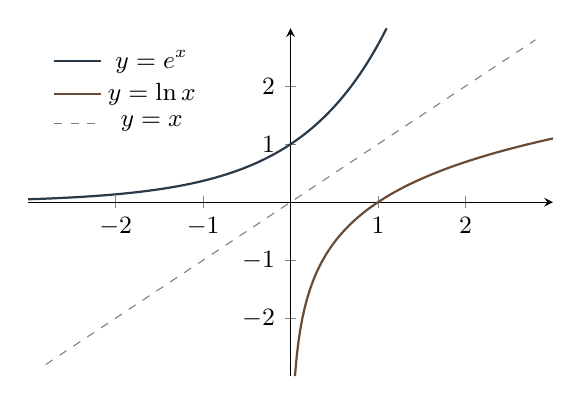
\begin{tikzpicture}
\begin{axis}[
width=0.68\linewidth,height=6cm,axis lines=middle,
xmin=-3,xmax=3,ymin=-3,ymax=3,
xtick={-2,-1,0,1,2},ytick={-2,-1,0,1,2},
tick label style={font=\small},legend style={draw=none,font=\small,at={(0.03,0.97)},anchor=north west}]
\addplot[deep,thick,domain=-3:1.0986,samples=140] {exp(x)};
\addlegendentry{$y=e^x$}
\addplot[accent,thick,domain=0.0498:3,samples=140] {ln(x)};
\addlegendentry{$y=\ln x$}
\addplot[gray,dashed,domain=-2.8:2.8] {x};
\addlegendentry{$y=x$}
\end{axis}
\end{tikzpicture}
\end{center}

图像反射立刻解释了前面已经得到的三条结构迁移：定义域和值域交换、点坐标交换、单调方向保持。

\subsubsection{对合函数：复合两次得到恒等映射}

如果 \(f:D\to D\) 是双射，那么

\[
\boxed{
f=f^{-1}
\Longleftrightarrow
f(f(x))=x,\quad x\in D.
}
\]

这样的函数也称为对合（involution）。例如

\[
f(x)=a-x
\]

在 \(\mathbb R\) 上满足 \(f(f(x))=x\)；

\[
f(x)=\frac1x
\]

在 \(\mathbb R\setminus\{0\}\) 上也满足 \(f(f(x))=x\)。它们的图像作为整体关于 \(y=x\) 反射以后不变。

\begin{warnbox}{图像坑：关于 \(y=x\) 对称，不代表两图只能在 \(y=x\) 上相交}
例如 \(f(x)=1-x\) 本身就是自己的反函数，所以 \(f\) 与 \(f^{-1}\) 的两条图像完全重合，其中绝大多数点并不在 \(y=x\) 上。

若额外知道 \(f\) 严格递增，则情况不同：若 \((a,b)\) 同时在 \(f\) 和 \(f^{-1}\) 图像上，就有 \(f(a)=b\)、\(f(b)=a\)。若 \(a<b\)，严格递增会推出 \(b=f(a)<f(b)=a\)，矛盾；\(a>b\) 同理。因此严格递增时共同点只能满足 \(a=b\)，即落在 \(y=x\) 上。
\end{warnbox}

在 \(f:D\to f(D)\) 单射、因而反函数存在的前提下，若 \(f\) 严格递增，则

\[
x_1<x_2
\Longrightarrow
f(x_1)<f(x_2),
\]

把输出重新视作反函数的输入即可得到 \(f^{-1}\) 也严格递增；严格递减的情形同理。因此

\[
\boxed{
\text{严格增}\leftrightarrow\text{反函数严格增},
\qquad
\text{严格减}\leftrightarrow\text{反函数严格减}.
}
\]

若定义域关于原点对称，且 \(f:D\to f(D)\) 单射并为奇函数，则

\[
f^{-1}(-y)=-f^{-1}(y),
\]

所以奇函数的反函数仍为奇函数。

更一般地，若 \(f:D\to f(D)\) 单射，并且 \(f\) 关于 \((a,b)\) 中心对称：

\[
f(2a-x)=2b-f(x),
\]

则

\[
f^{-1}(2b-y)=2a-f^{-1}(y),
\]

因此反函数关于 \((b,a)\) 中心对称。这正是中心坐标随
\((x,y)\mapsto(y,x)\) 一起交换。

\subsection{复合函数求逆为什么倒序？}

若

\[
g:A\to B,\qquad f:B\to C
\]

均为双射，则正向复合 \(f\circ g:A\to C\) 也是双射。要从 \(y\in C\) 回到 \(x\in A\)，必须先应用 \(f^{-1}\)，再应用 \(g^{-1}\)：

\[
y\xrightarrow{f^{-1}}u\xrightarrow{g^{-1}}x.
\]

因此

\[
\boxed{
(f\circ g)^{-1}=g^{-1}\circ f^{-1}.
}
\]

这里的``倒序''不是口诀，而是逆操作的时间顺序。立刻还得到

\[
\boxed{(f^{-1})^{-1}=f.}
\]

\subsubsection{仿射嵌套也只是复合求逆的展开}

设

\[
h(x)=A f(Bx+C)+D,
\qquad A\ne0,\ B\ne0,
\]

并设 \(f:I\to f(I)\) 为双射。令
\[
J=\{x\in\mathbb R:Bx+C\in I\},
\]
则 \(h:J\to h(J)\) 为双射。正向过程依次是

\[
x
\xrightarrow{Bx+C}
Bx+C
\xrightarrow{f}
f(Bx+C)
\xrightarrow{A(\cdot)+D}
y.
\]

逆过程必须倒序撤销：

\[
y
\xrightarrow{(y-D)/A}
\frac{y-D}{A}
\xrightarrow{f^{-1}}
f^{-1}\left(\frac{y-D}{A}\right)
\xrightarrow{(\cdot-C)/B}
x.
\]

所以

\[
\boxed{
h^{-1}(y)
=
\frac{f^{-1}\left(\frac{y-D}{A}\right)-C}{B},
\qquad y\in h(J).
}
\]

例如

\[
h(x)=2e^{3x-1}+4.
\]

取 \(f(u)=e^u\)，则 \(f^{-1}(u)=\ln u\)。于是

\[
\boxed{
h^{-1}(x)
=
\frac{1+\ln\left(\frac{x-4}{2}\right)}3,
\qquad x>4.
}
\]

这不是新的公式族，而是``复合求逆倒序''在坐标伸缩和平移中的具体展开。

\subsubsection{反函数符号不能像普通代数指数一样随意分配}

复合有明确的逆序规律，但点态加法、乘法一般没有类似分配律。通常不能写

\[
(f+g)^{-1}=f^{-1}+g^{-1}.
\]

例如取

\[
f(x)=x,
\qquad
g(x)=2x.
\]

则

\[
(f+g)(x)=3x,
\qquad
(f+g)^{-1}(x)=\frac x3,
\]

而

\[
f^{-1}(x)+g^{-1}(x)
=x+\frac x2
=\frac{3x}{2},
\]

显然不同。点态乘法同样不能凭符号形式推出``分别求逆再相乘''。原因是
\(^{-1}\) 在这里表示\textbf{映射的逆操作}，不是可以对任意代数运算分配的指数。

\subsection{两个可以直接判定非单射的结构}\label{ux4e24ux4e2aux91cdux8981ux7684ux4e0dux53efux9006ux4fe1ux53f7}

\begin{itemize}
\tightlist
\item
  若偶函数的定义域关于原点对称并同时含有某个 \(x\ne0\) 与 \(-x\)，则
  \(f(x)=f(-x)\)，不能单射；
\item
  非恒定周期函数在整个周期域上重复取值，也不能全局单射。
\end{itemize}

因此遇到偶函数、周期函数去求反函数，第一动作不是写
\(f^{-1}\)，而是先判断能否选择一个使限制映射单射的子域。限制定义域不是纯代数技巧，而是在重新指定一个可以建立逆映射的函数对象。

\begin{center}\rule{0.5\linewidth}{0.5pt}\end{center}

\section{统一结构语言：先找输入关系，再给性质命名}\label{ux7edfux4e00ux7ed3ux6784ux8bedux8a00ux5148ux627eux8f93ux5165ux5173ux7cfbux518dux7ed9ux6027ux8d28ux547dux540d}

\subsection{反射}\label{ux53cdux5c04}

关于 \(x=a\) 的反射记为

\[
R_a(x)=2a-x.
\]

讨论任何反射结构以前，先检查定义域是否对该反射封闭：

\[
x\in D\Longrightarrow 2a-x\in D.
\]

\subsubsection{轴对称}\label{ux8f74ux5bf9ux79f0}

若

\[
\boxed{f(2a-x)=f(x)},
\]

则图像关于直线 \(x=a\) 轴对称。

\subsubsection{中心对称}\label{ux4e2dux5fc3ux5bf9ux79f0}

若

\[
\boxed{f(2a-x)=2b-f(x)},
\]

则图像关于点 \((a,b)\) 中心对称。

把中心移到原点：

\[
g(u)=f(a+u)-b,
\]

就得到

\[
g(-u)=-g(u).
\]

因此一般中心对称不是另一套孤立公式，而是\textbf{平移后的奇结构}。

\subsection{奇偶性只是反射结构的特殊位置}\label{ux5947ux5076ux6027ux53eaux662fux53cdux5c04ux7ed3ux6784ux7684ux7279ux6b8aux4f4dux7f6e}

\subsubsection{偶函数}\label{ux5076ux51fdux6570}

当 \(a=0\) 时，轴对称退化为

\[
\boxed{f(-x)=f(x)}.
\]

所以偶函数就是关于 \(y\) 轴对称的函数。

\subsubsection{奇函数}\label{ux5947ux51fdux6570}

当 \((a,b)=(0,0)\) 时，中心对称退化为

\[
\boxed{f(-x)=-f(x)}.
\]

若 \(0\in D\)，则必有

\[
f(0)=0.
\]

\subsubsection{边界}\label{ux8fb9ux754c}

\begin{itemize}
\tightlist
\item
  定义域不关于原点对称时，不谈通常意义下的奇偶性；
\item
  零函数同时是奇函数和偶函数；
\item
  ``不是偶函数''不能推出``没有轴对称''，因为对称轴可能在 \(x=a\ne0\)；
\item
  ``不是奇函数''也不能推出``没有中心对称''，中心可能不在原点。
\end{itemize}

\subsection{第四问的平移分支：固定平移下函数值满足什么关系？}\label{ux5e73ux79fb}

前文四问母模型中的第四问研究\textbf{输入关系在映射下的保持与变换}。这里固定输入关系为“相差一个常数 \(L\)”，即 \(x_2=x_1+L\)，考察对应函数值之间的关系。

平移记为

\[
\tau_L(x)=x+L.
\]

面对一个固定平移量 \(L\)，第一步不是先给它贴上``周期''或``半周期''标签，而是比较

\[
f(x+L)\quad\text{与}\quad f(x)
\]

之间究竟存在什么稳定关系。以下讨论默认相应平移保持定义域合法；若把它作为全局平移结构，最清楚的集合写法是

\[
D+L=D.
\]

对第四问而言，现在固定输入变换为 \(x\mapsto x+L\)，再比较 \(f(x+L)\) 与 \(f(x)\) 的函数值关系。常见情形可以分成三类：

\begin{enumerate}
\tightlist
\item
  \textbf{直接恢复}：\(f(x+L)=f(x)\)。这时 \(L\) 本身就是周期；
\item
  \textbf{翻转}：\(f(x+L)=2b-f(x)\)。一次平移没有恢复，但同样的平移再做一次会恢复，因此能够生成周期；
\item
  \textbf{纵向漂移}：\(f(x+L)=f(x)+C\)。重复平移会累积漂移，一般不会产生周期。
\end{enumerate}

因此，这一节只是“四问母模型 → 第四问 → 固定平移下的函数值关系”的局部展开。\textbf{周期由 \(f(x+T)=f(x)\) 定义；翻转关系与漂移关系则是另外两类平移函数值关系。} 它们不应被写成三个并列定义。

\subsubsection{周期：一次平移直接恢复}\label{ux5468ux671f}

若某个 \(T\ne0\) 满足

\[
D+T=D,
\qquad
\boxed{f(x+T)=f(x)},
\]

则 \(T\) 是 \(f\) 的一个周期。

一个周期不等于最小正周期。存在周期也不保证一定存在``最小的''正周期。

\subsubsection{平移翻转关系：迭代两次可推出周期}\label{ux5e73ux79fbux7ffbux8f6c}

若存在常数 \(b\)，使

\[
\boxed{f(x+L)=2b-f(x)},
\]

那么平移 \(L\) 后，输出不是恢复原值，而是变成关于水平线 \(y=b\) 的对称值。令

\[
g(x)=f(x)-b,
\]

便得到

\[
g(x+L)=-g(x).
\]

把同样的平移再作用一次：

\[
\begin{aligned}
f(x+2L)
&=2b-f(x+L)\\
&=2b-[2b-f(x)]\\
&=f(x).
\end{aligned}
\]

所以

\[
\boxed{f(x+L)=2b-f(x)\Longrightarrow 2L\text{ 是一个周期}.}
\]

把同一关系连续使用两次便得到 $f(x+2L)=f(x)$。因此该翻转关系能够推出周期，但它本身不是周期的另一种定义。

当 \(b=0\) 时，翻转关系退化为

\[
f(x+L)=-f(x),
\]

即平移以后输出反号。这只是上述翻转现象关于基准线 \(y=0\) 的特殊情况。

\begin{warnbox}{为什么不把 \(L\) 默认叫``半周期''？}
由 \(f(x+L)=-f(x)\) 只能推出 \(2L\) 是\textbf{一个周期}，不能推出 \(2L\) 就是最小正周期。因此仅凭反号关系，还不足以证明 \(L\) 是最小正周期的一半。

例如 \(f(x)=\sin x\) 的最小正周期是 \(2\pi\)，但
\[
\sin(x+\pi)=-\sin x,
\qquad
\sin(x+3\pi)=-\sin x.
\]
\(\pi\) 是最小正周期的一半，而 \(3\pi\) 同样产生反号，却显然不是``半个最小周期''。只有进一步证明 \(2L\) 恰好就是最小正周期时，才可以把 \(L\) 解释为该最小正周期的一半。
\end{warnbox}

反向同样不能成立：知道 \(2L\) 是周期，并不能推出

\[
f(x+L)=-f(x)
\]

或更一般的 \(f(x+L)=2b-f(x)\)。

\subsubsection{平移漂移：有稳定关系也不等于周期}\label{ux5e73ux79fbux6f02ux79fb}

若

\[
f(x+L)=f(x)+C,
\]

则连续做 \(n\) 次同样的平移得到

\[
f(x+nL)=f(x)+nC.
\]

只要 \(C\ne0\)，输出就会持续累积纵向漂移，而不是恢复原值。因此``存在稳定的平移关系''并不自动等于周期；周期要求的是输出真正恢复。

\begin{center}\rule{0.5\linewidth}{0.5pt}\end{center}

\section{任意函数的奇偶分解：没有纯结构时，主动把结构拆出来}\label{ux4efbux610fux51fdux6570ux7684ux5947ux5076ux5206ux89e3ux6ca1ux6709ux7eafux7ed3ux6784ux65f6ux4e3bux52a8ux628aux7ed3ux6784ux62c6ux51faux6765}

只要定义域关于原点对称，对任意函数 \(f\) 定义

\[
f_e(x)=\frac{f(x)+f(-x)}2,
\]

\[
f_o(x)=\frac{f(x)-f(-x)}2.
\]

则

\[
\boxed{f(x)=f_e(x)+f_o(x)},
\]

其中 \(f_e\) 为偶函数，\(f_o\) 为奇函数。

而且这个分解是唯一的。

\subsection{为什么唯一？}\label{ux4e3aux4ec0ux4e48ux552fux4e00}

假设还有

\[
f=e_1+o_1=e_2+o_2,
\]

其中 \(e_1,e_2\) 偶，\(o_1,o_2\) 奇，则

\[
e_1-e_2=o_2-o_1.
\]

左边是偶函数，右边是奇函数；一个函数若同时奇且偶，只能是零函数，因此

\[
e_1=e_2,\qquad o_1=o_2.
\]

这里应理解为\textbf{代数上的唯一拆分}。在当前数学一语境中，不额外引入``正交投影''之类需要函数空间和内积结构的语言。

这个分解以后会通过 H-B01 与对称区间积分、Fourier
等模块发生接口，但分解本身由专题01拥有。

\begin{center}\rule{0.5\linewidth}{0.5pt}\end{center}

\section{坐标变换：结构没有消失，只是位置和尺度变了}\label{ux5750ux6807ux53d8ux6362ux7ed3ux6784ux6ca1ux6709ux6d88ux5931ux53eaux662fux4f4dux7f6eux548cux5c3aux5ea6ux53d8ux4e86}

考虑

\[
g(x)=A f(Bx+C)+D,
\]

先讨论非退化情形 \(A\ne0,B\ne0\)。

最稳的理解不是背``左加右减、上加下减''，而是拆成两层：

\begin{enumerate}
\def\labelenumi{\arabic{enumi}.}
\tightlist
\item
  内部变量 \[
  u=Bx+C
  \] 决定横向位置与尺度；
\item
  外部变换 \[
  y\mapsto Ay+D
  \] 决定纵向尺度、翻转与基准线。
\end{enumerate}

\subsection{定义域先变}\label{ux5b9aux4e49ux57dfux5148ux53d8}

若 \(f\) 的定义域为 \(D_f\)，则

\[
\boxed{D_g=\{x:Bx+C\in D_f\}}.
\]

所有后续结构都必须在这个新定义域上讨论。

\subsection{对称轴}\label{ux5bf9ux79f0ux8f74}

若 \(f(u)\) 关于 \(u=a\) 轴对称，则令

\[
Bx+C=a
\]

得到 \(g\) 的对应对称轴

\[
\boxed{x=\frac{a-C}{B}}.
\]

\subsection{对称中心}\label{ux5bf9ux79f0ux4e2dux5fc3}

若 \(f(u)\) 关于 \((a,b)\) 中心对称，则 \(g\) 关于

\[
\boxed{\left(\frac{a-C}{B},Ab+D\right)}
\]

中心对称。

\subsection{周期}\label{ux5468ux671f-1}

若 \(T\) 是 \(f\) 的一个周期，则使内部变量改变 \(T\) 即可：

\[
B\Delta x=T.
\]

因此 \(T/B\) 是一个带方向的平移量，而对应的正周期长度为

\[
\boxed{\frac{\lvert T\rvert}{\lvert B\rvert}}.
\]

若 \(T_0>0\) 是最小正周期，则在当前非退化条件 \(A\ne0,B\ne0\) 下，\(g\) 的最小正周期为

\[
\boxed{\frac{T_0}{\lvert B\rvert}}.
\]

若 \(A=0\)，则 \(g\) 在自己的定义域 \(D_g\) 上取常值 \(D\)，但周期性仍取决于 \(D_g\) 的平移不变性，不能由 \(f\) 的周期直接推出最小正周期。若 \(B=0\) 且 \(f(C)\) 有定义，则 \(D_g=\mathbb R\) 且 \(g\) 为常函数；此时每个非零实数都是周期，所以不存在最小正周期。

\begin{center}\rule{0.5\linewidth}{0.5pt}\end{center}

\section{结构怎样在函数代数内部组合？}\label{ux7ed3ux6784ux600eux6837ux5728ux51fdux6570ux4ee3ux6570ux5185ux90e8ux7ec4ux5408}

这一节仍然属于
专题01，因为操作两侧都是函数对象本身；一旦操作换成极限、求导、积分、展开，就切换到
H-B01。

\subsection{奇偶性的符号代数}\label{ux5947ux5076ux6027ux7684ux7b26ux53f7ux4ee3ux6570}

在定义域合法的前提下：

\[
\text{偶}\pm\text{偶}=\text{偶},\qquad
\text{奇}\pm\text{奇}=\text{奇},
\]

\[
\text{偶}\cdot\text{偶}=\text{偶},\qquad
\text{奇}\cdot\text{奇}=\text{偶},\qquad
\text{奇}\cdot\text{偶}=\text{奇}.
\]

除法在分母不为零且定义域保持对称时遵循同样的符号逻辑。

真正的生成机制只有一句：

\begin{quote}
对 \(x\mapsto -x\) 做代换，逐层追踪每个因子带来的 \(+1/-1\) 符号。
\end{quote}

所以不需要把每一条单独死记。

\subsection{主动构造奇偶结构}\label{ux4e3bux52a8ux6784ux9020ux5947ux5076ux7ed3ux6784}

对任意定义域关于原点对称的 \(f\)：

\[
f(x)+f(-x)\quad\text{一定是偶函数},
\]

\[
f(x)-f(-x)\quad\text{一定是奇函数}.
\]

另外，若复合有定义：

\[
f(\lvert x\rvert)
\]

一定是偶函数，因为 \(\lvert -x\rvert=\lvert x\rvert\)。

\subsection{周期函数组合先找公共周期}\label{ux5468ux671fux51fdux6570ux7ec4ux5408ux5148ux627eux516cux5171ux5468ux671f}

若同一个 \(T\) 同时是 \(f,g\) 的周期，则

\[
f\pm g,\qquad fg
\]

仍以 \(T\) 为周期；商还需保证分母不为零。

因此组合周期的核心不是``最小公倍数''这个词，而是：

\[
\boxed{\text{能否找到一个共同平移，使所有分量同时恢复原值？}}
\]

如果只知道两个最小正周期比值为无理数，不能对完全一般的函数机械写出``和一定非周期''；只能说不能从这两个周期直接构造公共整数倍周期。

\subsection{复合函数先看内层输入关系}\label{ux590dux5408ux51fdux6570ux5148ux770bux5185ux5c42ux8f93ux5165ux5173ux7cfb}

设

\[
h(x)=f(g(x)).
\]

若内函数满足

\[
g(-x)=g(x),
\]

则只要复合有定义，就有

\[
h(-x)=f(g(-x))=f(g(x))=h(x),
\]

所以

\[
\boxed{\text{内偶}\Rightarrow\text{复合函数必偶}.}
\]

外函数不需要是偶函数。

若 \(g\) 为奇函数，则继续观察外函数是否满足

\[
f(-u)=\pm f(u).
\]

于是得到

\[
\text{偶}\circ\text{奇}=\text{偶},\qquad
\text{奇}\circ\text{奇}=\text{奇}.
\]

令 \(h=f\circ g\)。若 \(T\ne0\)、复合定义域满足 \(D_h+T=D_h\)，并且对所有 \(x\in D_h\) 有

\[
g(x+T)=g(x),
\]

则

\[
f(g(x+T))=f(g(x)),
\]

所以 \(T\) 是 \(h\) 的一个周期。

但复合函数的周期也可能由外函数的周期性产生。若 \(T\) 是外函数 \(f\) 的周期，并存在 \(P\ne0\) 使 \(D_h+P=D_h\)，且

\[
g(x+P)=g(x)+kT,\qquad k\in\mathbb Z
\]

对所有 \(x\in D_h\) 成立，则

\[
f(g(x+P))=f(g(x)+kT)=f(g(x)),
\]

所以 \(P\) 也是复合函数的一个周期。此时内函数 \(g\) 本身完全可以不是周期函数。

这些都是\textbf{充分条件}，不是反向等价判据；复合函数还可能因为外函数的非单射性、偶性或周期性而具有比内函数更强的结构。统一动作仍是：\textbf{先写出内函数在目标输入变换下的等式，再把该等式代入外函数，直接比较复合前后的函数值。}

\begin{center}\rule{0.5\linewidth}{0.5pt}\end{center}

\section{两次反射为什么会生成周期？}\label{ux4e24ux6b21ux53cdux5c04ux4e3aux4ec0ux4e48ux4f1aux751fux6210ux5468ux671f}

这是专题01中最值得保留的一条生成性关系。

定义

\[
R_a(x)=2a-x,
\qquad
R_b(x)=2b-x.
\]

连续做两次反射：

\[
R_b(R_a(x))
=2b-(2a-x)
=x+2(b-a).
\]

所以

\[
\boxed{R_b\circ R_a=\text{平移 }2(b-a)}.
\]

也就是说：

\[
\boxed{\text{两次反射}=\text{一次平移}.}
\]

\subsection{两个对称轴}\label{ux4e24ux4e2aux5bf9ux79f0ux8f74}

若 \(f\) 同时关于 \(x=a\) 与 \(x=b\)
轴对称，\(a\ne b\)，则两次反射后函数值仍不变，因此

\[
\boxed{2\lvert b-a\rvert\text{ 是 }f\text{ 的一个周期}.}
\]

\subsection{两个同高度的对称中心}\label{ux4e24ux4e2aux540cux9ad8ux5ea6ux7684ux5bf9ux79f0ux4e2dux5fc3}

若 \(f\) 分别关于 \((a,c)\) 与 \((b,c)\)
中心对称，\(a\ne b\)，连续使用两次中心对称关系后函数值恢复，于是得到

\[
\boxed{2\lvert b-a\rvert\text{ 是一个周期}.}
\]

\subsection{一个轴 + 一个中心}\label{ux4e00ux4e2aux8f74-ux4e00ux4e2aux4e2dux5fc3}

若

\[
f(2a-x)=f(x),
\]

同时

\[
f(2b-x)=2c-f(x),
\]

则

\[
\boxed{f(x+2(b-a))=2c-f(x)}.
\]

也就是说，先得到平移翻转关系；把同一等式再使用一次，函数值恢复：

\[
\boxed{4\lvert b-a\rvert\text{ 是一个周期}},\qquad a\ne b.
\]

若 \(a=b\)，同一横坐标既是对称轴又是中心横坐标，则条件强迫

\[
f(x)\equiv c,
\]

此时不能把 \(0\) 当作通常意义上的正周期。

\subsection{周期怎样反过来复制已有对称结构？}

前面是``两个反射生成平移''。反过来，一旦已经知道一个周期，还可以把一条已知对称轴或一个已知对称中心平移到新的对称位置。

若 \(T\) 是 \(f\) 的一个周期，且 \(x=a\) 是一条对称轴，则

\[
f(2a-x)=f(x).
\]

考察横坐标 \(a+T/2\)：

\[
\begin{aligned}
f\left(2\left(a+\frac T2\right)-x\right)
&=f(2a+T-x)\\
&=f(2a-x)\\
&=f(x).
\end{aligned}
\]

所以 \(a+T/2\) 也是对称轴。重复使用周期得到

\[
\boxed{x=a+\frac{kT}{2},\qquad k\in\mathbb Z}
\]

都是对称轴。

同理，若 \(f\) 关于 \((a,b)\) 中心对称，即

\[
f(2a-x)=2b-f(x),
\]

则

\[
\boxed{\left(a+\frac{kT}{2},b\right),\qquad k\in\mathbb Z}
\]

也都是中心对称点。

这给出一条很有生成力的双向图：

\[
\boxed{
\text{两条已知反射对称条件}
\Longrightarrow
\text{平移关系}
\Longrightarrow
\text{结合已知对称轴/中心推出同类对称的一族}
}
\]

注意最后一步必须先有至少一条已知对称轴或一个已知对称中心；\textbf{周期性本身不能推出函数存在轴对称或中心对称。} 例如
\[
f(x)=\sin x+\sin 2x
\]
以 \(2\pi\) 为周期，但不存在竖直对称轴。若假设 \(x=a\) 是对称轴，则必须对所有 \(t\) 有 \(f(a+t)=f(a-t)\)，于是
\[
2\cos a\sin t+2\cos 2a\sin 2t=0.
\]
这要求 \(\cos a=0\) 与 \(\cos2a=0\) 同时成立，而二者不可能同时成立。这个最小反例专门阻断“有周期 \(\Rightarrow\) 必有对称轴”的误推。

\subsection{拓展关系：不同高度中心产生``平移 + 漂移''}\label{extensionux4e0dux540cux9ad8ux5ea6ux4e2dux5fc3ux4ea7ux751fux5e73ux79fb-ux6f02ux79fb}

若中心分别为 \((a,c_1)\) 与 \((b,c_2)\)，则

\[
\boxed{f(x+2(b-a))=f(x)+2(c_2-c_1)}.
\]

只有 \(c_1=c_2\) 时才退化为真正的周期。

这条关系先作为专题01的结构拓展保留；它以后会与 H-B01
中``周期函数的原函数可能发生线性漂移''形成接口，但这里不展开积分机制。

\begin{center}\rule{0.5\linewidth}{0.5pt}\end{center}

\section{单调、有界与单射：不是所有结构都来自对称}\label{ux5355ux8c03ux6709ux754cux4e0eux5355ux5c04ux4e0dux662fux6240ux6709ux7ed3ux6784ux90fdux6765ux81eaux5bf9ux79f0}

反射和平移描述的是``相关输入之间函数值怎样对应''。函数还有另外三类非常基础的结构。

\subsection{单调性：输入顺序怎样传到输出}\label{ux5355ux8c03ux6027ux8f93ux5165ux987aux5e8fux600eux6837ux4f20ux5230ux8f93ux51fa}

在区间 \(I\) 上，若对任意 \(x_1<x_2\)：

\begin{itemize}
\tightlist
\item
  总有 \(f(x_1)\le f(x_2)\)，则 \(f\) 单调不减；
\item
  总有 \(f(x_1)\ge f(x_2)\)，则 \(f\) 单调不增；
\item
  若始终为严格不等号，则分别为严格递增、严格递减。
\end{itemize}

因此单调性的核心关系是

\[
\boxed{\text{输入的序关系}\longrightarrow\text{输出的序关系}.}
\]

本册只拥有这个结构定义及其与单射/反函数存在性的关系；怎样由 \(f'\)
的符号得到单调区间，由 Topic04 拥有。

\subsection{单射性：不同输入能否被输出区分}\label{ux5355ux5c04ux6027ux4e0dux540cux8f93ux5165ux80fdux5426ux88abux8f93ux51faux533aux5206}

单射要求

\[
f(x_1)=f(x_2)\Longrightarrow x_1=x_2.
\]

它回答的是：对每个给定输出，原像是否唯一，也就是函数是否单射。

严格单调函数在区间上一定单射，因此可以在值域上建立反函数。

但``单射''与``单调''不是同一个定义；尤其在非区间或离散定义域上，不能把二者直接等同。

\subsection{有界性：输出能否被一个固定范围控制}\label{ux6709ux754cux6027ux8f93ux51faux80fdux5426ux88abux4e00ux4e2aux56faux5b9aux8303ux56f4ux63a7ux5236}

例如在集合 \(D\) 上若存在 \(M\) 使

\[
\lvert f(x)\rvert\le M,\qquad \forall x\in D,
\]

则称 \(f\) 在 \(D\) 上有界。

有界性描述的是\textbf{值域整体被限制在某个有限范围内}，不是局部变化快慢，也不等于连续。$\operatorname{sgn}x$ 在 $0$ 处间断但有界；$1/x$ 在 $(0,1)$ 上连续却无界，所以“有没有间断点”不是判断有界性的直接判据。

连续函数为什么在闭区间有界、开区间在有限端点极限下为什么仍有界、有限区间上有界导数为什么给出函数有界等结论，由专题04借助紧致性/中值定理拥有其证明；连续周期函数怎样把单周期有界性复制到全局则由 H-B01 负责。

\subsection{结构联用：周期 + 全局单调}\label{ux7ed3ux6784ux8054ux7528ux5468ux671f-ux5168ux5c40ux5355ux8c03}

若 \(f\) 在整个实轴上具有非零周期，同时又全局单调，则 \(f\)
只能是常函数。

原因不是微分，而是两个结构直接冲突：

\begin{itemize}
\tightlist
\item
  单调性要求随着输入顺序持续保持输出顺序；
\item
  周期性要求相隔一个周期以后输出重新回到原值。
\end{itemize}

这是一条纯粹的专题01结构联用结论。

\begin{center}\rule{0.5\linewidth}{0.5pt}\end{center}

\section{概念边界：真正要分清的不是名词，而是判据}\label{ux6982ux5ff5ux8fb9ux754cux771fux6b63ux8981ux5206ux6e05ux7684ux4e0dux662fux540dux8bcdux800cux662fux5224ux636e}

{\def\LTcaptype{none} % do not increment counter
\begin{longtable}[]{@{}
  >{\raggedright\arraybackslash}p{(\linewidth - 8\tabcolsep) * \real{0.1765}}
  >{\centering\arraybackslash}p{(\linewidth - 8\tabcolsep) * \real{0.2941}}
  >{\raggedright\arraybackslash}p{(\linewidth - 8\tabcolsep) * \real{0.1765}}
  >{\raggedright\arraybackslash}p{(\linewidth - 8\tabcolsep) * \real{0.1765}}
  >{\raggedright\arraybackslash}p{(\linewidth - 8\tabcolsep) * \real{0.1765}}@{}}
\toprule\noalign{}
\begin{minipage}[b]{\linewidth}\raggedright
概念边界
\end{minipage} & \begin{minipage}[b]{\linewidth}\raggedright
为什么会混淆
\end{minipage} & \begin{minipage}[b]{\linewidth}\raggedright
真正区别
\end{minipage} & \begin{minipage}[b]{\linewidth}\raggedright
题目信号
\end{minipage} & \begin{minipage}[b]{\linewidth}\raggedright
混淆后果
\end{minipage} \\
\midrule\noalign{}
\endhead
\bottomrule\noalign{}
\endlastfoot
函数表达式 vs 函数对象 & 同一个解析式很容易让人误以为对象已经确定 &
函数对象还包含定义域与逐点对应，表达式只是表示 & 看到约分、开方、对数、补定义时先查定义域 &
把不同定义域的对象当成同一个函数 \\
陪域 vs 值域 & 在基础微积分里常把目标集合省略，于是两个词容易被当成同义 &
陪域是映射声明允许输出落入的目标集合 \(B\)；值域是实际到达的 \(f(D)\subseteq B\) & 题目出现满射、双射、\(f:D\to B\) 或问反函数定义域时恢复这一区分 &
把“实际能取到”与“声明允许取到”混在一起，进而误判满射或反函数的定义域 \\
隐式关系 \(F(x,y)=0\) vs 单值函数 \(y=f(x)\) & 二者都用 \(x,y\) 描述关系 &
函数要求每个允许的 \(x\) 只对应一个 \(y\) & 圆、闭曲线、平方后出现多支时先查竖线是否只交一次 &
对不存在的全局函数直接求反函数或套函数性质 \\
表示变换 vs 对象等价 & 代数等式常让人忽略变形前后的对象信息 &
等价表示必须保持合法输入、逐点输出、分支与覆盖信息 & 平方、约分、消元、参数化时检查增解、漏解与定义域 &
新表达式算得对，但已经不是原问题 \\
偶函数 vs 一般轴对称 & 偶函数确实是一种轴对称，容易把特殊位置当成全部情况 &
偶函数只对应轴 \(x=0\)，一般轴为 \(x=a\) & 出现 \(f(a+x)=f(a-x)\) 时识别一般轴 &
看到``非偶''就误判为``无对称'' \\
奇函数 vs 一般中心对称 & 奇函数确实是一种中心对称，容易把原点当成唯一中心 &
奇函数中心固定在 \((0,0)\)，一般中心满足 \(f(a+x)+f(a-x)=2b\) &
条件中同时出现平移后的两个镜像输入时寻找 \((a,b)\) & 漏掉水平/竖直平移后的奇结构 \\
一个周期 vs 最小正周期 & 若 \(T\) 是周期，则任意非零整数倍 \(nT\) 仍是周期 &
\(f(x+T)=f(x)\) 只说明 \(T\) 是周期，最小正周期还需排除更小正值 & 题目出现``最小''时必须继续做最小性检查 &
把 \(2T,3T\) 等直接当基本周期 \\
周期关系 vs 平移翻转关系 & 两者都比较 $f(x+L)$ 与 $f(x)$，所以容易混淆 &
周期要求一次平移后输出直接恢复；翻转则把输出送到关于某条水平线的对称值，必须再作用一次才恢复 & 出现 \(f(x+L)=f(x)\)、\(f(x+L)=2b-f(x)\) 或 \(f(x+L)=-f(x)\) 时直接按等式判断 &
把翻转步长 \(L\) 直接叫周期/半周期，或由 \(2L\) 是周期反推平移 \(L\) 必然反号 \\
反函数 \(f^{-1}\) vs 倒数 \(1/f\) & 上标 \(-1\) 容易被误读成普通负指数 &
反函数恢复输入并要求单射；倒数只对函数值取倒数并要求 \(f\ne0\) &
看到 \(f^{-1}(y)=x\) 时先改写为 \(f(x)=y\) & 公式、定义域和值域全部错位 \\
反函数存在 vs 能写成熟悉闭式 & 两个问题在``求反函数''题目中常被一起出现 &
存在性只取决于映射能否唯一倒回；闭式写法取决于当前表示与允许工具 & 已证单射但方程仍难以孤立 \(x\) 时分开判断 &
因为不会显式反解就误判为不存在反函数 \\
候选代数根 vs 合法反函数分支 & 开方、平方、二次方程都会自然产生多个候选 &
反函数必须同时满足原定义域、符号/分支条件并保持唯一性 & 出现 \(\pm\)、平方、\(t=e^x>0\) 时回到原对象筛支 &
把 \(\pm\) 直接写进反函数，或保留不可能的根 \\
全局三角函数 vs 主值反三角函数 & \(\arcsin,\arccos,\arctan\) 的名字容易让人以为它们能撤销整个周期函数 &
反三角函数只逆转指定的双射主值分支；原三角函数在完整定义域上非单射 & 出现 \(\arcsin(\sin x)\)、\(\arccos(\cos x)\)、\(\arctan(\tan x)\) 时先检查内层输入是否落在主值区间 &
把主值代表映射误写成全局恒等式 \\
\(g^{-1}\!\circ g\) vs \(g^{-1}\!\circ F\) & 形式上都像“反函数套原函数” &
前者要求内层就是被求逆的同一个双射 \(g\)；若 \(F\) 是在较大定义域上非单射的延拓，则复合只返回主值代表 & 正弦、余弦、正切先区分“全局函数”与“限制后的主支” &
错误写出 \(\arcsin(\sin x)=x\) 对所有实数成立 \\
\(x=f^{-1}(y)\) vs \(y=f^{-1}(x)\) & 都出现同一个 \(f^{-1}\) 记号 &
前者与 \(y=f(x)\) 描述同一组点 \((x,y)\)；后者是把变量角色重命名后得到的反函数图像 & 题目问“哪些式子同义、哪些图像关于 \(y=x\) 对称”时先分关系表示与函数图像 &
把同一关系和镜像图像混成一件事 \\
\(\sec,\csc,\cot\) vs 反三角函数 & 倒数关系和“反”字在中文里容易靠得很近 &
\(\sec=1/\cos\)、\(\csc=1/\sin\)、\(\cot=1/\tan\) 是倒数；\(\arctan,\operatorname{arccot}\) 才是选定分支的映射逆 & 看到上标 \(-1\)、arc、sec/csc 时先判断是在取倒数还是求映射逆 &
把正割/余割或余切误当成反函数 \\
单调不减/不增 vs 严格单调 & 中文资料有时笼统写“单调函数有反函数” &
严格单调可保证区间上单射；非严格单调可以有平台区间 & 遇到“单调函数有反函数”先确认教材术语是否把单调定义成严格意义 &
把常函数等非严格单调函数误判为存在反函数 \\
单射 vs 严格单调 & 在区间题中二者常一起出现 &
单射问不同输入能否被输出区分；严格单调还要求保持或反转输入顺序 & 区间上严格单调可作为单射的充分条件，但不要反过来改定义 &
把单射/反函数存在条件机械改写成导数或单调条件 \\
局部结构 vs 全局结构 & 同一个解析式在不同区间可以表现出不同结构 &
在一个区间上单调或限制映射存在反函数，不代表整个定义域都成立 & 反三角、周期函数、隐函数出现时先确认当前分支 &
把局部分支误当全局反函数 \\
\end{longtable}
}

\begin{center}\rule{0.5\linewidth}{0.5pt}\end{center}

\section{与后续专题的接口}\label{ux4e0eux540eux7eed-topic-ux7684ux63a5ux53e3}

专题01的任务是\textbf{定义结构本身}。当题目开始问``这种结构经过某种微积分操作以后会怎样''，就应停止在本册继续堆公式，转入相应知识归属。

{\def\LTcaptype{none} % do not increment counter
\begin{longtable}[]{@{}
  >{\raggedright\arraybackslash}p{(\linewidth - 4\tabcolsep) * \real{0.3333}}
  >{\raggedright\arraybackslash}p{(\linewidth - 4\tabcolsep) * \real{0.3333}}
  >{\raggedright\arraybackslash}p{(\linewidth - 4\tabcolsep) * \real{0.3333}}@{}}
\toprule\noalign{}
\begin{minipage}[b]{\linewidth}\raggedright
当前信号
\end{minipage} & \begin{minipage}[b]{\linewidth}\raggedright
本册提供
\end{minipage} & \begin{minipage}[b]{\linewidth}\raggedright
后续归属
\end{minipage} \\
\midrule\noalign{}
\endhead
\bottomrule\noalign{}
\endlastfoot
偶/奇/一般对称函数在对称点附近求极限 & 给出反射关系与合法定义域 &
Topic02 + H-B01 \\
连续严格单调函数的反函数是否连续、反函数极限怎样研究 & 给出所选双射限制、定义域/值域交换与 \(f^{-1}(y)=x\Longleftrightarrow f(x)=y\) & Topic02 + H-B01 \\
对称函数求导后结构怎样变 & 给出原函数对称关系 & Topic03 + H-B01 \\
对称/周期函数做定积分、原函数、变上限积分 & 给出原结构 & Topic05 +
H-B01 \\
对称条件怎样影响单调、极值、函数形状 & 给出对称/单调结构语义 &
Topic04 \\
奇偶性怎样筛掉 Taylor / Fourier 系数 & 给出奇偶结构 & Topic11 + H-B01 \\
反函数在对应点的导数、二阶导数或局部形状怎样求 & 给出 \(f^{-1}(y)=x\Longleftrightarrow f(x)=y\) 的对象关系与合法分支 & Topic03 + H-B01 \\
\end{longtable}
}

核心归属规则：

\[
\boxed{
\text{专题01定义“结构是什么”}
\quad;
\quad
\text{H-B01 定义“结构经过别的机制后怎样传播”}.
}
\]

\begin{center}\rule{0.5\linewidth}{0.5pt}\end{center}

\section{调用接口与训练路由}\label{ux9898ux76eeux8c03ux7528ux534fux8bae}

专题01正文只保留最小调用接口：

\[
\boxed{
\text{确认对象}
\to
\text{选择能保留信息的表示}
\to
\text{测试输入变换/原像数量}
\to
\text{读取结构}
\to
\text{独立检查}
}
\]

如果目标是求反函数，再切换为

\[
\boxed{
\text{判单射/限制分支}
\to
\text{确定原值域}
\to
\text{恢复输入}
\to
\text{恢复合法分支}
\to
\text{复合验证}
}.
\]

具体母题、变式、反解表示、主值代表映射、局部规则与检查动作不再在正文重复展开；统一由本专题 README 导航到同目录的\textbf{函数对象与定义域、函数表示与信息保护、基本函数结构、复合函数、反函数、反三角主值与复合、对称性、周期性、值域与单射、单调性}训练文档。若题目开始研究极限、求导、积分或展开后的结构传播，则切换到 H-B01 与对应专题。

\begin{center}\rule{0.5\linewidth}{0.5pt}\end{center}

\section{\texorpdfstring{贯穿母例：\(g(x)=2\cos(3x-1)+4\)}{贯穿母例：g(x)=2\textbackslash cos(3x-1)+4}}\label{ux8d2fux7a7fux6bcdux4f8bgx2cos3x-14}

这个例子故意同时包含平移、伸缩、周期、对称、基准线，以及“在整个 \(\mathbb R\) 上非单射”这一结构。

\subsection{先确认对象}\label{ux5148ux786eux8ba4ux5bf9ux8c61}

\[
g:\mathbb R\to\mathbb R,
\qquad
g(x)=2\cos(3x-1)+4.
\]

定义域为

\[
D_g=\mathbb R,
\]

值域为

\[
[2,6].
\]

\subsection{换表示，而不是直接硬看长式}\label{ux6362ux8868ux793aux800cux4e0dux662fux76f4ux63a5ux786cux770bux957fux5f0f}

令

\[
u=3x-1.
\]

于是

\[
g(x)=2\cos u+4.
\]

现在横向结构都先在 \(u\) 中读取，再通过 \(u=3x-1\) 解回
\(x\)；纵向基准线由 \(+4\) 决定。

\subsection{周期}\label{ux5468ux671f-2}

\(\cos u\) 的最小正周期为 \(2\pi\)，所以

\[
3\Delta x=2\pi
\]

得到

\[
\boxed{T=\frac{2\pi}{3}}.
\]

\subsection{对称轴}\label{ux5bf9ux79f0ux8f74-1}

\(\cos u\) 关于

\[
u=k\pi
\]

轴对称，因此

\[
3x-1=k\pi,
\]

即

\[
\boxed{x=\frac{1+k\pi}{3}},\qquad k\in\mathbb Z.
\]

\subsection{对称中心}\label{ux5bf9ux79f0ux4e2dux5fc3-1}

\(\cos u\) 关于

\[
\left(\frac\pi2+k\pi,0\right)
\]

中心对称；外部变换把中心高度 \(0\) 送到 \(4\)，因此 \(g\) 的中心为

\[
\boxed{
\left(
\frac{1+\frac\pi2+k\pi}{3},
4
\right)
},\qquad k\in\mathbb Z.
\]

\subsection{平移以后围绕基准线翻转}\label{ux5e73ux79fbux7ffbux8f6cux6bcdux4f8b}

内部平移 \(\pi\) 时

\[
\cos(u+\pi)=-\cos u.
\]

对应 \(x\) 平移 \(\pi/3\)：

\[
g\left(x+\frac\pi3\right)
=4-2\cos(3x-1)
=8-g(x).
\]

所以真正结构是

\[
\boxed{g\left(x+\frac\pi3\right)=8-g(x)},
\]

即函数值围绕基准线 \(y=4\) 翻转。这不是周期定义本身；把同一关系再使用一次可得 $g(x+2\pi/3)=g(x)$，因此 $2\pi/3$ 是周期。也不能简单写成 \(g(x+\pi/3)=-g(x)\)，因为基准线并不在 \(y=0\)。

\subsection{为什么没有全局反函数？}\label{ux4e3aux4ec0ux4e48ux6ca1ux6709ux5168ux5c40ux53cdux51fdux6570}

因为 \(g\) 是非恒定周期函数，同一个函数值会无限重复出现，所以它在
\(\mathbb R\) 上不是单射。

若限制到

\[
3x-1\in[0,\pi],
\]

即

\[
x\in\left[\frac13,\frac{1+\pi}{3}\right],
\]

此时 \(\cos u\) 在该区间严格递减，\(g\) 也严格递减，因此该限制映射单射，并且在其实际值域上存在反函数。

由

\[
y=2\cos(3x-1)+4
\]

得到

\[
\cos(3x-1)=\frac{y-4}{2},
\]

在选定分支上

\[
3x-1=\arccos\frac{y-4}{2},
\]

所以

\[
\boxed{
g^{-1}(y)=
\frac{1+\arccos\left(\frac{y-4}{2}\right)}{3}
},
\qquad y\in[2,6].
\]

\subsubsection{母例暴露的典型错误}\label{ux6bcdux4f8bux66b4ux9732ux7684ux5178ux578bux9519ux8bef}

如果一看到

\[
y=2\cos(3x-1)+4
\]

就直接``移项 + arccos''，会误以为得到整个周期函数的全局反函数。

真正缺失的不是代数步骤，而是 \textbf{对象 → 单射性 → 分支}
这一层对象检查。

\begin{center}\rule{0.5\linewidth}{0.5pt}\end{center}

\section{章节 / 考纲映射}\label{ux7ae0ux8282-ux8003ux7eb2ux6620ux5c04}

传统教材中下列内容由本册重新组织：

\begin{itemize}
\tightlist
\item
  函数概念、定义域、值域；
\item
  基本初等函数与函数表示；
\item
  分段函数；
\item
  复合函数；
\item
  反函数的存在性、分支选择、典型构造、反三角主值区间与主值代表映射；
\item
  隐式与参数表示的对象边界；
\item
  单调、有界、奇偶、周期等基础性质；
\item
  一般对称与坐标变换下的结构识别。
\end{itemize}

但以下传统上也常与``函数性质''一起出现的内容，本册只提供接口，不重新拥有：

\begin{itemize}
\tightlist
\item
  连续性与极限；
\item
  导数判单调、极值、凹凸；
\item
  对称区间积分；
\item
  变上限积分；
\item
  Taylor / Fourier 中的奇偶筛选。
\end{itemize}

正文按认知归属组织，考纲目录只用于覆盖检查。

\begin{center}\rule{0.5\linewidth}{0.5pt}\end{center}

\section{错误模式应该定位到哪里？}\label{ux9ad8ux9891ux9519ux8befux5e94ux8be5ux5b9aux4f4dux5230ux54eaux91cc}

专题01只保留一条诊断原则：表面算错以后，不停在“粗心”或“这题不会”，而要回到

\[
\boxed{
\text{对象}\to\text{表示}\to\text{输入合法性/输入关系}\to\text{输出关系}\to\text{结构/反解}\to\text{验证}
}
\]

寻找第一次偏离有效推理的位置。完整错误路由、典型错法与对应训练入口已经移入同目录《常见错误与断点定位》，避免 Canonical 再维护一份题型错误百科。


\section{一页压缩}\label{ux4e00ux9875ux538bux7f29}

\subsection{一句话}\label{ux4e00ux53e5ux8bdd}

\[
\boxed{
\text{函数不是解析式；先确定函数对象，再用四问定位定义域、像集、单射性与关系型结构。}
}
\]

\subsection{总坐标系与分析协议}\label{ux4e00ux5f20ux6bcdux56fe}

\textbf{四问是总坐标系。} 下面这条链只是分析关系型结构时使用的执行协议，不是另一套与四问并列的母模型：

\[
\boxed{
\text{对象}
\to
\text{表示}
\to
\text{合法输入关系}
\to
\text{输出关系}
\to
\text{结构}
}
\]

\begin{itemize}
\tightlist
\item
  \textbf{对象}：定义域 + 对应规律；讨论满射/双射时恢复陪域；
\item
  \textbf{表示}：显式 / 分段 / 隐式 / 参数 / 图像；
\item
  \textbf{输入关系}：反射、平移、顺序、相等性；
\item
  \textbf{输出关系}：相等、反号、和为常数或保持/反转序关系；
\item
  \textbf{结构}：由这些输入—输出关系识别对称、奇偶、周期、单调等关系型结构。
\end{itemize}

总坐标系由\textbf{观察同一个函数对象的四个并列问题}构成，不是必须依次执行的四步流程：

\[
\boxed{
\begin{array}{ll}
\text{输入合法性} & x\in D\ ?\\[2mm]
\text{输出可达性} & y\in f(D)\ ?\\[2mm]
\text{原像唯一性} & \lvert f^{-1}(\{y\})\rvert\text{ 是多少？}\\[2mm]
\text{输入关系的映射规律} & x_1\,R_D\,x_2\Rightarrow f(x_1)\,R_B\,f(x_2)\ ?
\end{array}
}
\]

题目可以直接进入其中任意一问，不需要先完成前三问再讨论第四问。定义域、值域/有界性、单射/反函数，以及奇偶/对称/周期/单调，分别主要落在这四个观察维度。

\subsection{五个最重要的不变量}\label{ux56dbux4e2aux6700ux91cdux8981ux7684ux4e0dux53d8ux91cf}

\begin{enumerate}
\def\labelenumi{\arabic{enumi}.}
\tightlist
\item
  变形前后的合法输入不能被无意改变；
\item
  保留下来的输入必须对应同一个输出；
\item
  分支、覆盖与一一对应信息不能被偷偷丢掉；
\item
  结构判断必须建立在定义域对相应输入变换合法的前提上；
\item
  写 \(f^{-1}\circ f=I\) 或 \(f\circ f^{-1}=I\) 时，两边的 \(f\) 必须是\textbf{同一个已经指定定义域/值域的双射对象}；较大定义域上的非单射延拓不能替代所选双射分支。
\end{enumerate}

\subsection{核心生成关系}\label{ux4e09ux6761ux751fux6210ux5173ux7cfb}

\[
\boxed{\text{定义域}=\text{所有定义条件的交集}}
\]

\[
\boxed{\text{复合结构判断}=\text{内函数的变换关系}+\text{外函数在对应变换下的函数值关系}}
\]

\[
\boxed{\text{奇偶}=\text{原点处的反射结构}}
\]

\[
\boxed{\text{两次反射}=\text{一次平移}}
\]

\[
\boxed{f(x+L)=2b-f(x)\Rightarrow f(x+2L)=f(x)}
\]

这里表示平移翻转迭代两次生成周期，不表示 \(L\) 已经被证明是最小正周期的一半。

\[
\boxed{\text{已有周期}+\text{已知对称轴/中心}\Rightarrow\text{推出同类对称轴/中心的一族}}
\]

\[
\boxed{f:D\to f(D)\text{ 存在反函数}\Longleftrightarrow f\text{ 在 }D\text{ 上单射}}
\]

\[
\boxed{
\text{反三角函数}
=
\text{周期三角函数限制到主值单射分支以后再求逆}
}
\]

\[
\boxed{
\text{主值反函数}\circ\text{原全局三角函数}
=
\text{主值代表映射，而不是自动恒等}
}
\]

\[
\boxed{
\text{求反函数}
=
\text{判单射/分支}
\to
\text{确定值域}
\to
\text{选表示反解}
\to
\text{恢复合法分支}
\to
\text{复合验证}
}
\]

\subsection{重建问题}\label{ux91cdux5efaux95eeux9898}

忘掉具体公式时，依次问：

\begin{enumerate}
\def\labelenumi{\arabic{enumi}.}
\tightlist
\item
  当前真正的函数对象是什么，定义域有没有被省略？若式子含根式、对数、分母、反三角或复合，所有定义条件的交集是什么？
\item
  目标问的是值域/满射/反函数吗？若是，哪些输出实际可达，同一个输出有几个合法原输入，陪域与值域是否需要区分？
\item
  现在看到的是对象本身，还是对象的一种表示？
\item
  换表示以后有没有增解、漏解、丢分支或改变定义域？
\item
  题目正在比较哪两个输入：\(x\) 与 \(-x\)、\(2a-x\)、\(x+T\)，还是
  \(x_1<x_2\)？
\item
  这两个输入对应的函数值满足什么稳定关系？
\item
  能否因此识别轴、中心、奇偶、周期、单调或单射？
\item
  如果是复合函数，目标输入变换下 $g(\phi(x))$ 与 $g(x)$ 有什么关系？代入外函数后，$f(g(\phi(x)))$ 与 $f(g(x))$ 有什么关系？
\item
  如果同时给出两个反射结构，它们复合以后产生什么平移？若已经有周期和一条已知对称轴或一个已知对称中心，还能推出哪些同类对称轴/中心？
\item
  如果要求反函数，当前定义域是否单射；若不单射，应该限制到哪个分支？
\item
  写成 \(y=f(x)\) 后，哪一种表示最适合恢复 \(x\)：直接移项、指数换元、共轭、开方、反三角还是逐段反解？
\item
  反解产生的候选根是否都满足原定义域、符号和分支条件；反函数定义域是否等于原值域？
\item
  如果看到 \(\arcsin,\arccos,\arctan\)，对应的主值区间是什么？当前内层函数真的是那个被限制后的双射吗，还是全局周期函数？
\item
  如果是 \(\arcsin(\sin x)\) 一类式子，当前任务是恒等恢复还是把输入折回主值区间？如果是 \(\cos(\arcsin x)\) 一类式子，主值区间怎样决定根号正负？
\item
  如果开始求极限、导数、积分或展开，是否应该切换到 H-B01 与对应专题？
\end{enumerate}

只要这些问题还能回答，专题01
 的主干就能重新生成出来，而不需要把函数性质拆成一张孤立的公式表。

\end{document}
